\section{Shellcode} \label{sec:shellcode}
\subsection{Definition}
Um das folgende Beispiel besser zu verstehen, sollte zunächst erklärt werden, was genau Shellcode ist und wofür er benutzt wird.
Shellcode ist definiert als eine Folge von Anweisungen, die über einen Exploit in einen Prozess injiziert und
dann durch diesen ausgeführt werden. Er wird verwendet, um die Funktionalität eines Prozesses zu verändern und
Befehle auf einem Zielsystem auszuführen. In der Computersicherheit bedeutet Shellcoding im ursprünglichen Sinne
das Schreiben von Code, der bei der Ausführung eine Remote Shell öffnet. Die Bedeutung von Shellcode hat sich jedoch weiterentwickelt und
beschreibt mittlerweile jeden Byte Code, der in einen Exploit eingefügt wird, um eine gewünschte Aufgabe zu erfüllen.

Zwar ist es theoretisch möglich, Shellcode in höheren Programmiersprachen zu schreiben, in der Praxis ist die effizienteste und
fast ausschließlich verwendete Sprache jedoch Assembly. Der Einsatz Assembly ermöglicht, so maschinennah wie möglich zu arbeiten,
um mehr Kontrolle über Abläufe zu haben und Speicherplatz zu sparen. Der verfügbare Speicher für Shellcode ist meist limitiert.
Da Shellcode in Assembly geschrieben wird, ist es wichtig zu beachten, auf welcher Hardware und auf welchem Betriebssystem dieser laufen soll.
Es bestehen klare Unterschiede zwischen Linux und Windows Shellcode: Unter Linux hat man überwiegend direkten Zugriff auf Interface und Kernel,
was unter Windows in der Regel nicht möglich ist. Im Folgenden wird ein Shellcode-Beispiel für 64 Bit Unix Systeme betrachtet. \cite{tutorial1}

\subsection{Beispiel}

Der folgende Shellcode ermöglicht es, eine Shell auf dem ausführenden System zu öffnen und diese über eine Netzwerkverbindung fernzusteuern. 
Der Code umfasst dabei lediglich 29 Bytes, da dieser so effizient und klein wie möglich ist. 
Am besten lässt sich die Erklärung von hinten, also mit dem Syscall, beginnen.
Dieser ermöglicht es, auf unterschiedliche Funktionen des Betriebssystems zurückzugreifen und Befehle auszuführen. 
Um die Art des Syscalls festzulegen, muss eine Ganzzahl in das Register \codeline{rax} geladen werden. 
In diesem Fall wird zunächst die Hexadezimalzahl \codeline{0x42} geladen und das Register \codeline{ah}, 
welches ein 8 Bit Segment des 64 Bit \codeline{rax} Registers ist, inkrementiert. 
In \codeline{rax} befindet sich nun die Hexadezimalzahl \codeline{0x142} bzw. die Dezimalzahl \codeline{322}. 
Für den Syscall entspricht dieser Wert der Anweisung \codeline{execveat()}, 
die über einen Dateipfad angegebene Programme ausführt. Um den Syscall durchführen zu können, benötigt \codeline{execveat()} noch fünf Argumente, 
die über die Register \codeline{rdi}, \codeline{rdx}, \codeline{r10} und \codeline{r8} gesetzt werden. 
In \codeline{rdi} wird die Zeichenfolge \codeline{(''/bin//sh'')} als Hexadezimalzahl kodiert geladen. 
Zu beachten ist hierbei die invertierte Eingabe, da \codeline{execveat()} die Zeichenkette in Little-Endian-Reihenfolge erwartet. Das \codeline{rsp} Register, 
also der Stack Pointer, 
enthält nun einen Zeiger auf das \codeline{rdi} Register. Dieser Zeiger wird nun in das \codeline{rsi} Register geladen. Nun sind beide benötigten Argumente gesetzt. 
Abschließend werden die übrigen Argumente auf \codeline{0} gesetzt. Hierfür wird zunächst das \codeline{rdx} Register 
über \codeline{cqo} (convert word to quadword) auf \codeline{0} gesetzt und
anschließend der Wert von \codeline{rdx} in die Register \codeline{r10} und \codeline{r8} geschoben. 
Der Syscall kann nun erfolgreich durchgeführt werden und eine Shell öffnen. \cite{syscalls} \cite{execman}

\begin{figure}[h]
    \centering
    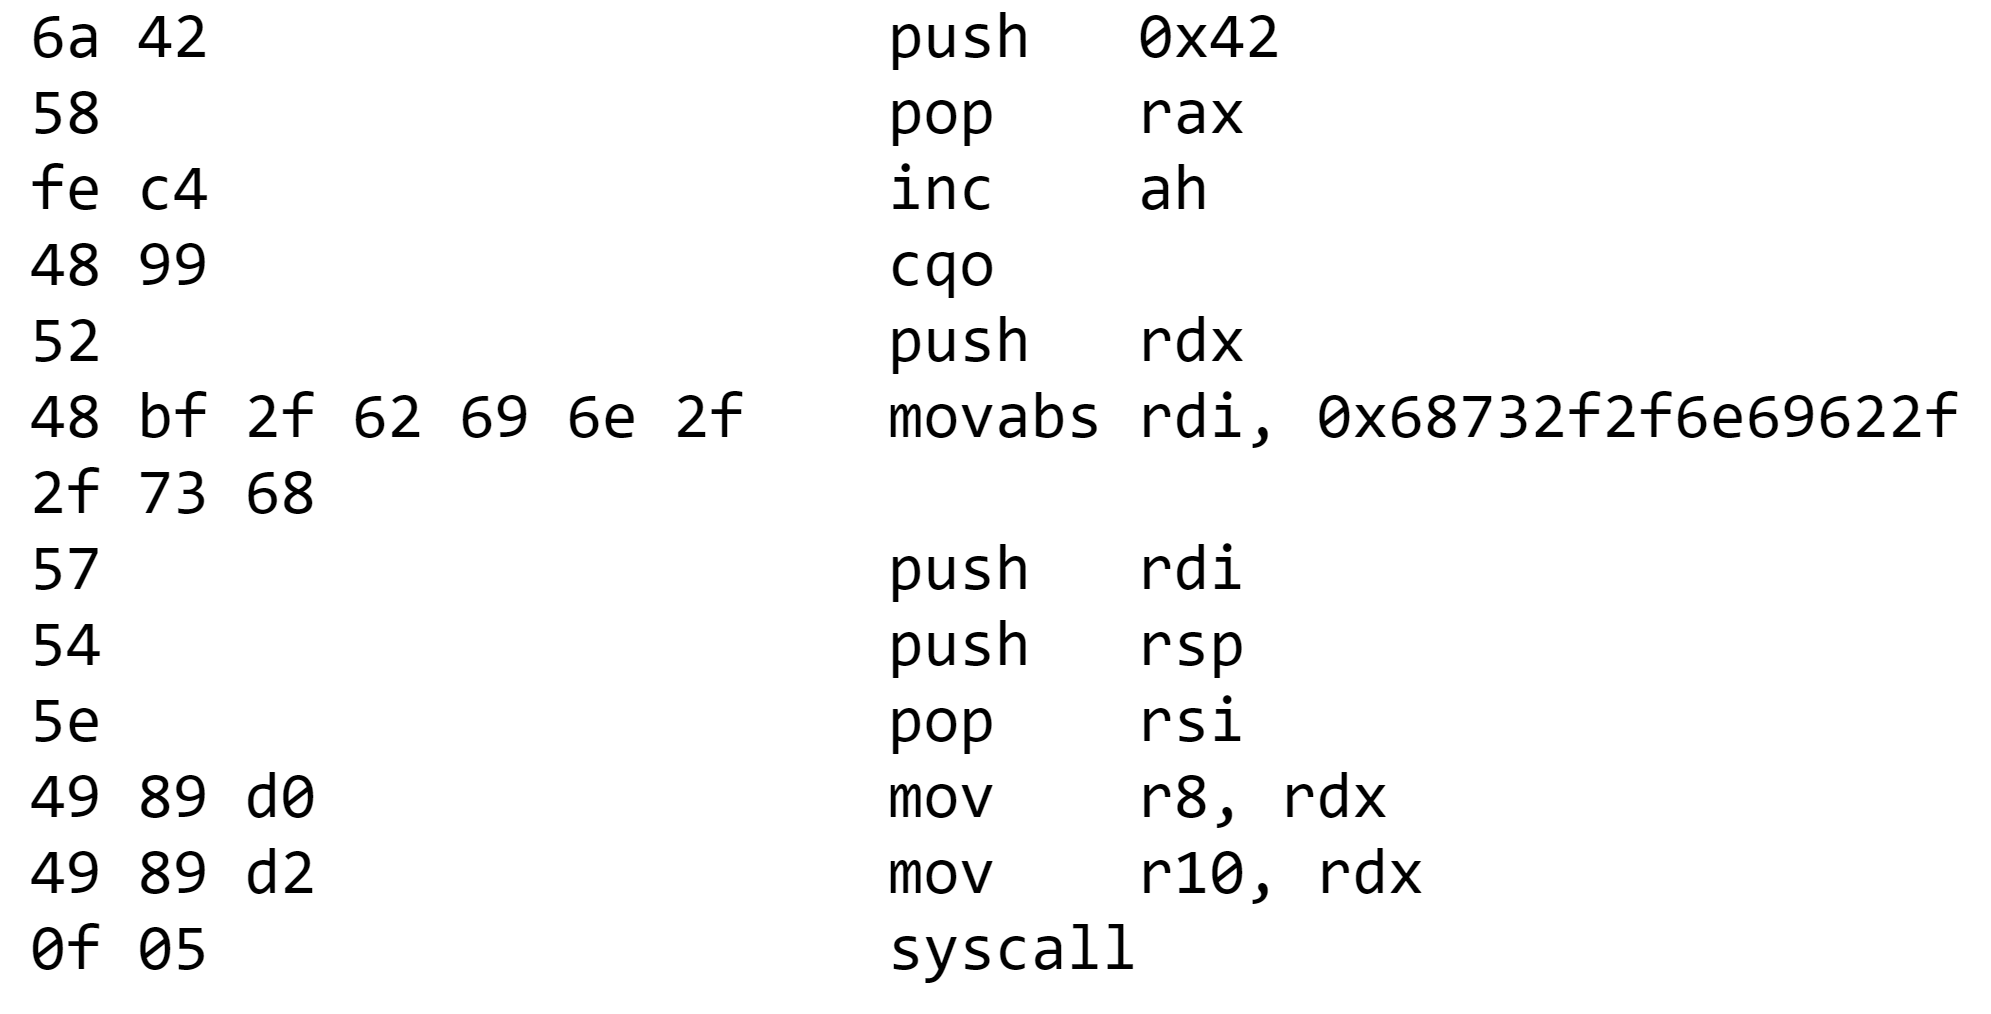
\includegraphics[width=0.9\textwidth,height=0.75\textheight,keepaspectratio]{images/shellstorm.png}
    \caption{Shellcode}
\end{figure}
\cite{shellstorm}

Die verwendeten Register und ihr Inhalt zum Zeitpunkt des Syscalls:

    \begin{tabular}{rl}
         {\textbf{RAX}:}& {322 (Nummer des Syscalls)}\\
         {\textbf{RDI}:}& {0x68732f2f6e69622f (Pfad der auszuführenden Datei: ''/bin//sh'')}\\
         {\textbf{RSI}:}& {Pointer auf RDI (Zeiger auf den Pfad)}
    \end{tabular}

    
Die optionalen bzw. nicht verwendeten Register zum Zeitpunkt des Syscalls:

    \begin{tabular}{rl}
        {\textbf{RDX}:}& {0 (Optional)}\\
        {\textbf{R10}:}& {0 (Optional)}\\
        {\textbf{R8}:}& {0 (Optional)}\\
        {\textbf{R9}:}& {? (Nicht verwendet)}
    \end{tabular}
    
